\chapter{November - 2012} % Chapter title
\label{ch:nov:2012} % For referencing the chapter elsewhere, use \autoref{ch:introduction}

%----------------------------------------------------------------------------------------------------

\section{SublimeText 2, disappear}
Today, I found the window of the program `SublimeText' disappeared. 
The window did not appear although I tried many times to restore it.
After a while, I found the reason. 
The multi-screen causes the SublimeText not to set its windows correctly. 
I can press the keys `<Win> + <Left Arrow>' to move it to the current screen.
\hfill {\tiny  edited on 2012-11-09.}

\section{Redhat, RHEL 6.2}
\subsection{Change, password, root}
In order to get familiar with Redhat 6.2, I installed it in the virtual machine by means of the Vmware.
However, I forget the password of the user 'root'.
After surfing the Internet, I found the solution. 
It can be reset through boot loader 'grub'.
After you see the boot menu, press 'e' to edit the boot item, like "kernel /vmlinuz-2. ro root".
You just append the word " single" on the item, and press 'b' to boot the machine.
You can login the linux OS as the user 'root'.
The command 'passwd' can change the password of 'root' without the old password.

\subsection{GUI from X windows to Multiuser}
You should edit the file '/etc/inittab', changing '5' into '3'.
For example, 'id:5:' to 'id:3:'.
After the system boots, the GUI interface will be changed into terminal window style.

\subsection{Configure, IP, eth0}
You edit the file '/etc/sysconfig/network-scripts/ifcfg-eth0' to set up the network interface of eth0.
For example, 
Device=eth0
BOOTPROTO=none
ONBOOT=yes
NETMASK=255.255.255.0
IPADDR=10.0.1.6
USERCTL=no

\url{https://access.redhat.com/knowledge/docs/en-US/Red_Hat_Enterprise_Linux/6/html/Deployment_Guide/s1-networkscripts-interfaces.html }
\hfill {\tiny  edited on 2012-11-13.}

\section{Samba, RHEL}
In order to restore the work environment, I install the samba server which can share files with the Windows OS clients.

The steps is shown in the following:
\begin{enumerate}[(1)]
\item Install samba server software in the RHEL 6.2.  you should execute the command as the user root: rpm -ivh samba-3.5.10-114.el6.i686.rpm
\item After installation, run the command 'rpm -q samba' to verify the samba server.
\item Go to the directory '/etc/samba', and find three files: smbusers, smb.conf, and lmhosts. For the file lmhosts, add the windows OS computer IP and name. For example,
\begin{verbatim}
        192.168.122.1 yanzw-PC
\end{verbatim}
For the file smbusers, add the user name. For example,
\begin{verbatim}
        username=lian
\end{verbatim}. 
For the file smb.conf, add the shared directory. For exmple, 
\begin{verbatim}
        [shared]
        path = /home/shared
        writeable = yes
        browseable = yes
        read only = No
        guest ok = Yes
        public = Yes
        valid users = yzw lian
        create mask = 0666
        directory mask = 0777
\end{verbatim}
\item run the commands:
\begin{verbatim}
    mkdir shared
    chmod a+w shared
    chcon -t samba_share_t shared
    useradd -c "PGSql Developer" -d /home/lian -s /sbin/nologin lian
    smbpasswd -a lian
   /sbin/service smb restart
   /sbin/service nmb restart
\end{verbatim}
\end{enumerate}
\hfill {\tiny  edited on 2012-11-15.}

\section{shared library, RHEL 6.2}
The command 'ldconfig' can refresh the library cache. 
If your program does not find the library, you should add your required library path into the system library path, modifying the file '/etc/ld.so.conf'.
\hfill {\tiny  edited on 2012-11-14.}

\section{PostgreSQL, Reading}
\subsection{Database Infransture}
The PostgreSQL runs as the mode 'Client/Server'. 
The program called "postgres" is the server process, which executes all commands of clients. It supports concurrent connections using 'fork()'.
The client programs submit their requests to the process 'postgres', and display the responses from the server.
\subsection{users}
PostgreSQL users are different from the Unix users.
You should add the specifical user for the database.
The server must be run by the PostgreSQL user account and not by root or any other user.
\subsection{Source, Installation}
You run the following commands as the user 'root'.
\begin{verbatim}
./configure
gmake
su
gmake install
\end{verbatim}

\subsection{Add user, directory of data}
You run the following commands as the user 'root'.
\begin{verbatim}
adduser postgres
mkdir /usr/local/pgsql/data
chown postgres /usr/local/pgsql/data
\end{verbatim}

\subsection{Initilize DB server, run DB server}
You run the following commands as the user 'root'.
\begin{verbatim}
su - postgres
/usr/local/pgsql/bin/initdb -D /usr/local/pgsql/data
/usr/local/pgsql/bin/postgres -D /usr/local/pgsql/data >logfile 2>&1 &
\end{verbatim}

\subsection{Create database example}
\begin{verbatim}
/usr/local/pgsql/bin/createdb test
/usr/local/pgsql/bin/psql test
=# select current_date;
=# \q
\end{verbatim}

\subsection{Template database}
There are two template databases, 'postgres' and 'template1'.

\subsection{Out of memory}
The memory parameters can be changed in the file '/etc/sysctl.conf'

\subsection{authentication}
pg\_hba.conf means host-based authentication.

\hfill {\tiny  edited on 2012-11-16.}


\section{Document, Writing, Rules}
\begin{enumerate}[(1)]
    \item All information should be recored in English in the jotting files.
    The jotting files are located in directory 
    \begin{verbatim}
    'c:\user\yanzw\desktop\my_jotting\'
    \end{verbatim}
    \item You should write the detail in English as possible as you can.
\end{enumerate}
\hfill {\tiny  edited on 2012-11-17.}


\section{Glog, SendMail}
\subsection{SendMail}
The SendMail is a Email program that send email via outside smtp server from a command line.
The command line options is shown in Fig. \ref{fig:send:mail:command}
You can download the program from 
\url{http://caspian.dotconf.net/menu/Software/SendEmail/}.

\begin{figure}[htbp]
\centering
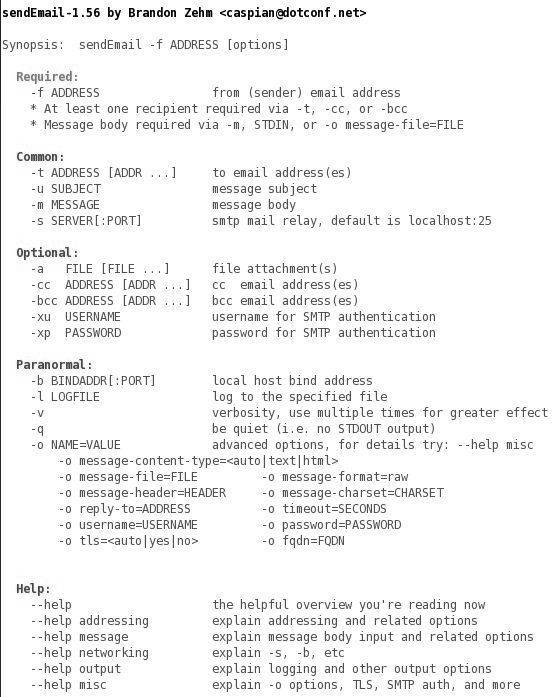
\includegraphics[width=0.95\textwidth]{./Chapters/pictures/sendEmail.jpg}
\caption{SendEmail}
\label{fig:send:mail:command}
\end{figure}
\hfill {\tiny  edited on 2012-11-09.}

\section{Venture lab, brainstorming}
\subsection{Room}
First, there has to be room for people walk around.
Second, there are space enough on a whiteboard to capture all the ideas.
\subsection{Participants}
The people should have different points of view and expertise on the topic.
They get together to collect all possibilities.
The policy of the size of group is 'two-pizza teams'.
\subsection{topic}
The question you ask is the frame into which the solution will fall.
\subsection{How to start a brainstorming session}
Maybe you can start with a seemingly silly prompt. For example, 'how would you design eyeglasses if we didn't have ears?'.
\subsection{Rules of brainstorming}
The participants aren't allowed to criticize ideas.
The key is to embrace all ideas that generated and to work with them for a while.
You must not evaluate ideas as they are generated.
It is also important to encourage wild and crazy ideas.
Even though they may seem strange, there may be a gem hidden inside.
Students can come up with the worst ideas they can during a brainstorming session.
When people are asked to generate bad ideas, they defer judgement and push beyond obvious solutions.
\subsection{Process of brainstorming}
One approach is to remove the most obvious solutions from the pool of possibilities, so that you have to come up with something new or strange.
Someone comes up with an idea, and several people build on it for a short time.
Then you jump to a new approach. 
The dance could be called 'build, build, build, Jump!'.
\subsection{Capture ideas}
Everyone has a pen and paper or sticky notes.
\subsection{Time}
It do not exceed more than one hour.
Maybe it is ten to fifteen minutes.
\subsection{Decision}
Everyone votes for all the ideas.

\subsection{Final step}
Take photos of all the ideas, make notes about the best ones, and save all the materials that can be saved.
As time goes by, some of the ideas that seem impractical might look promising.

\hfill {\tiny  edited on 2012-11-20.}

\section{RHEL 6.2 CDROM}
Question: I found the CDROM was not mounted automatically if I changed the GUI interface to Bash interface.
Solution: 
\begin{enumerate}[(1)]
    \item Create the directory: \begin{verbatim} mkdir \cdrom \end{verbatim} 
    \item Execute the command: \begin{verbatim} mount \dev\cdrom \cdrom \end{verbatim}
\end{enumerate}

\hfill {\tiny  edited on 2012-11-28.}

